\newpage
\section{Trabajo Extra Voluntario}
\label{sec:trabajo_extra}

En este apartado se detalla el trabajo extra realizado por el alumno. La estructura trata básicamente en exponer la motivación y descripción teórica, pseudocódigo, configuración experimental y análisis. Para ello se introducen aquí los resultados obtenidos y los boxplots correspondientes \footnote{Es de suma importancia mencionar que se han incluido los dos algoritmos extra implementados en la práctica 1. Aunque no se vayan a analizar en detalle debido a que esta parte ya se realizó en el informe anterior, se usarán para realizar ciertas comparaciones y exponer breves anotaciones y/o comentarios.}.

\subsection{Resultados Numéricos y Boxplots de los Extras}

\begin{table}[H]
\centering
\caption{Resultados extras -- IBEX 35}
\label{tab:extras-ibex35}
\resizebox{\textwidth}{!}{%
\begin{tabular}{lccccc}
\hline
Algoritmo & Fitness(2015--2024) & Fitness(2025) & Beneficio & Evaluaciones & Tiempo (s) \\
\hline
BL Best    & -4.712 & -3.169 &  0.037 &  9872 & 0.006 \\
BL Multi   & -4.564 & -3.104 &  0.024 & 10000 & 0.008 \\
AGG-Gauss  & -4.511 & -3.102 &  0.035 & 10000 & 0.009 \\
AM-LSCh    & -4.490 & -3.082 &  0.033 &  9953 & 0.009 \\
DE         & -4.491 & -3.083 &  0.033 & 10000 & 0.012 \\
\hline
\end{tabular}
}
\end{table}

\begin{table}[H]
\centering
\caption{Resultados extras -- S\&P 100}
\label{tab:extras-sp100}
\resizebox{\textwidth}{!}{%
\begin{tabular}{lccccc}
\hline
Algoritmo & Fitness(2015--2024) & Fitness(2025) & Beneficio & Evaluaciones & Tiempo (s) \\
\hline
BL Best    & -3.855 & -4.500 & 0.073 & 10000 & 0.065 \\
BL Multi   & -3.044 & -3.868 & 0.095 & 10000 & 0.077 \\
AGG-Gauss  & -2.938 & -3.742 & 0.093 & 10000 & 0.072 \\
AM-LSCh    & -2.791 & -3.743 & 0.107 & 10000 & 0.073 \\
DE         & -2.807 & -3.758 & 0.108 & 10000 & 0.081 \\
\hline
\end{tabular}
}
\end{table}

\begin{table}[H]
\centering
\caption{Resultados extras -- S\&P 500}
\label{tab:extras-sp500}
\resizebox{\textwidth}{!}{%
\begin{tabular}{lccccc}
\hline
Algoritmo & Fitness(2015--2024) & Fitness(2025) & Beneficio & Evaluaciones & Tiempo (s) \\
\hline
BL Best    & -4.272 & -5.002 & 0.009 & 10000 & 1.439 \\
BL Multi   & -3.385 & -4.295 & 0.003 & 10000 & 1.603 \\
AGG-Gauss  & -2.880 & -3.934 & 0.021 & 10000 & 1.447 \\
AM-LSCh    & -2.761 & -3.888 & 0.017 &  9968 & 1.478 \\
DE         & -2.717 & -3.885 & 0.019 & 10000 & 1.495 \\
\hline
\end{tabular}
}
\end{table}

\begin{figure}[H]
    \centering
    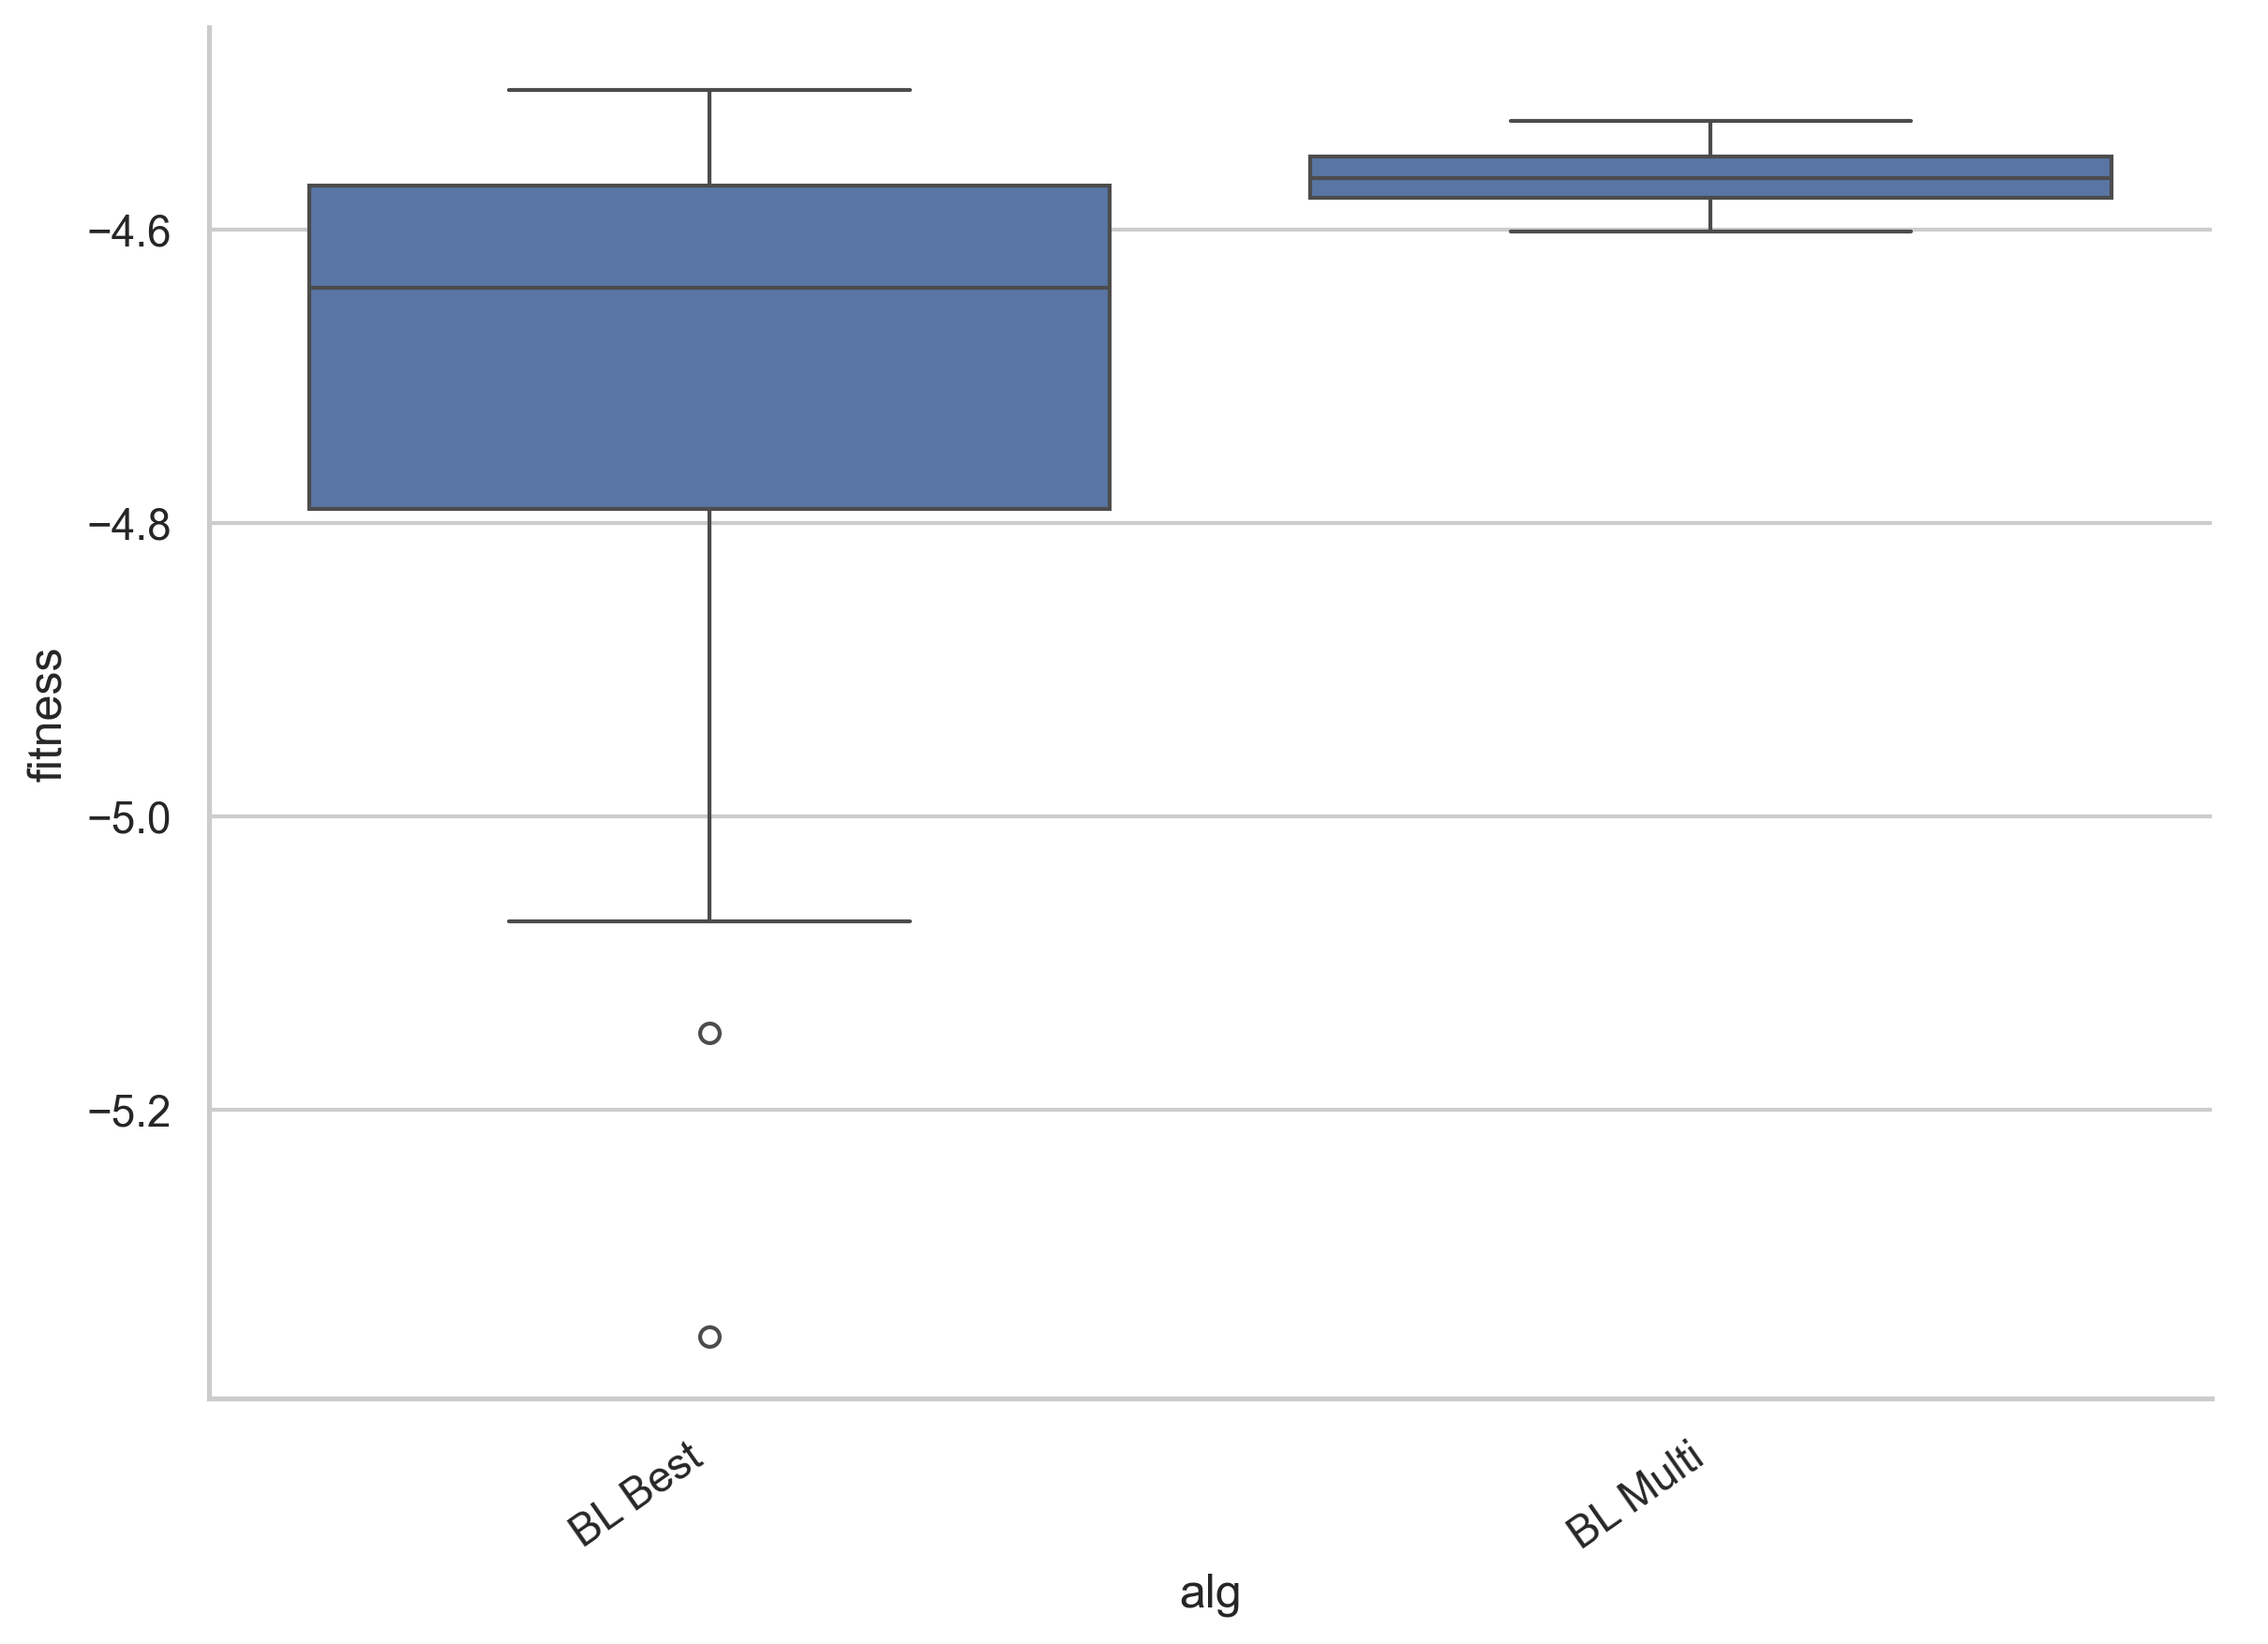
\includegraphics[width=0.85\textwidth]{figuras/IBEX_35_RESULTS_pr1_extras.png}
    \caption{Boxplots de los extras de la Práctica 1 -- IBEX 35 (BL Best y BL Multi).}
    \label{fig:pr1-extras-ibex}
\end{figure}

\begin{figure}[H]
    \centering
    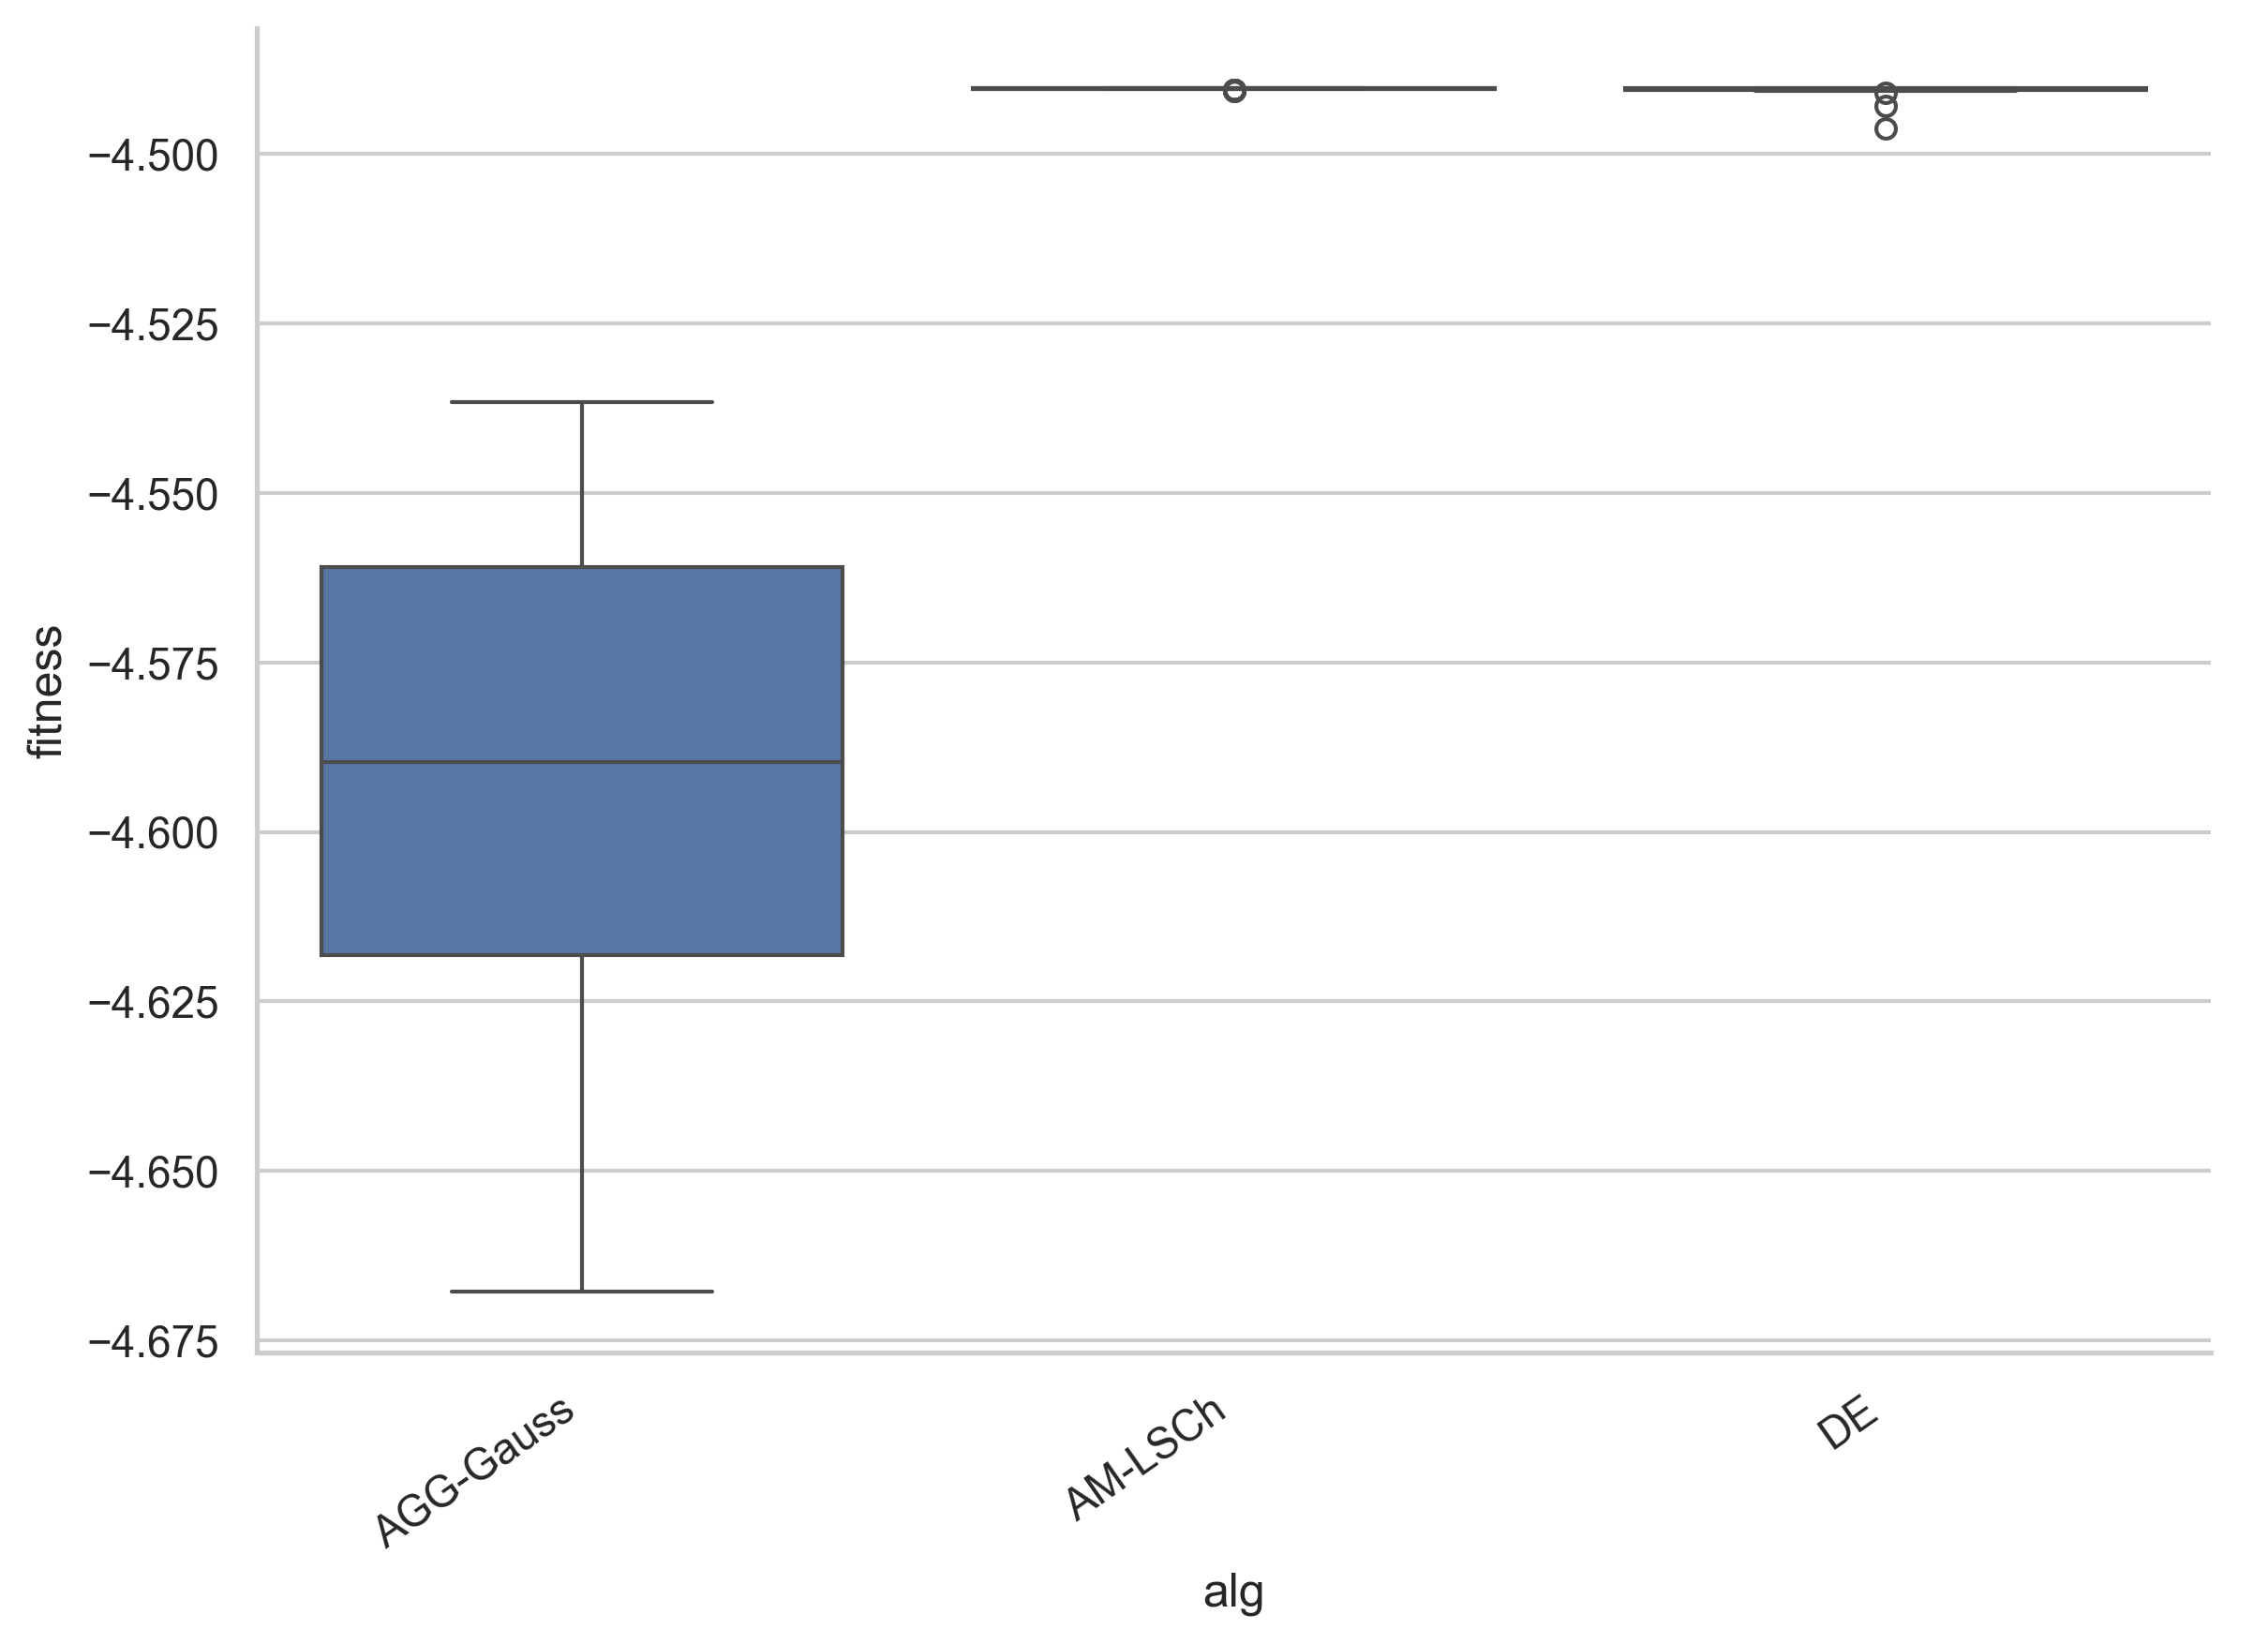
\includegraphics[width=0.85\textwidth]{figuras/IBEX_35_RESULTS_pr2_extras.png}
    \caption{Boxplots de los extras de la Práctica 2 -- IBEX 35 (AGG-Gauss, AM-LSCh y DE).}
    \label{fig:pr2-extras-ibex}
\end{figure}

\begin{figure}[H]
    \centering
    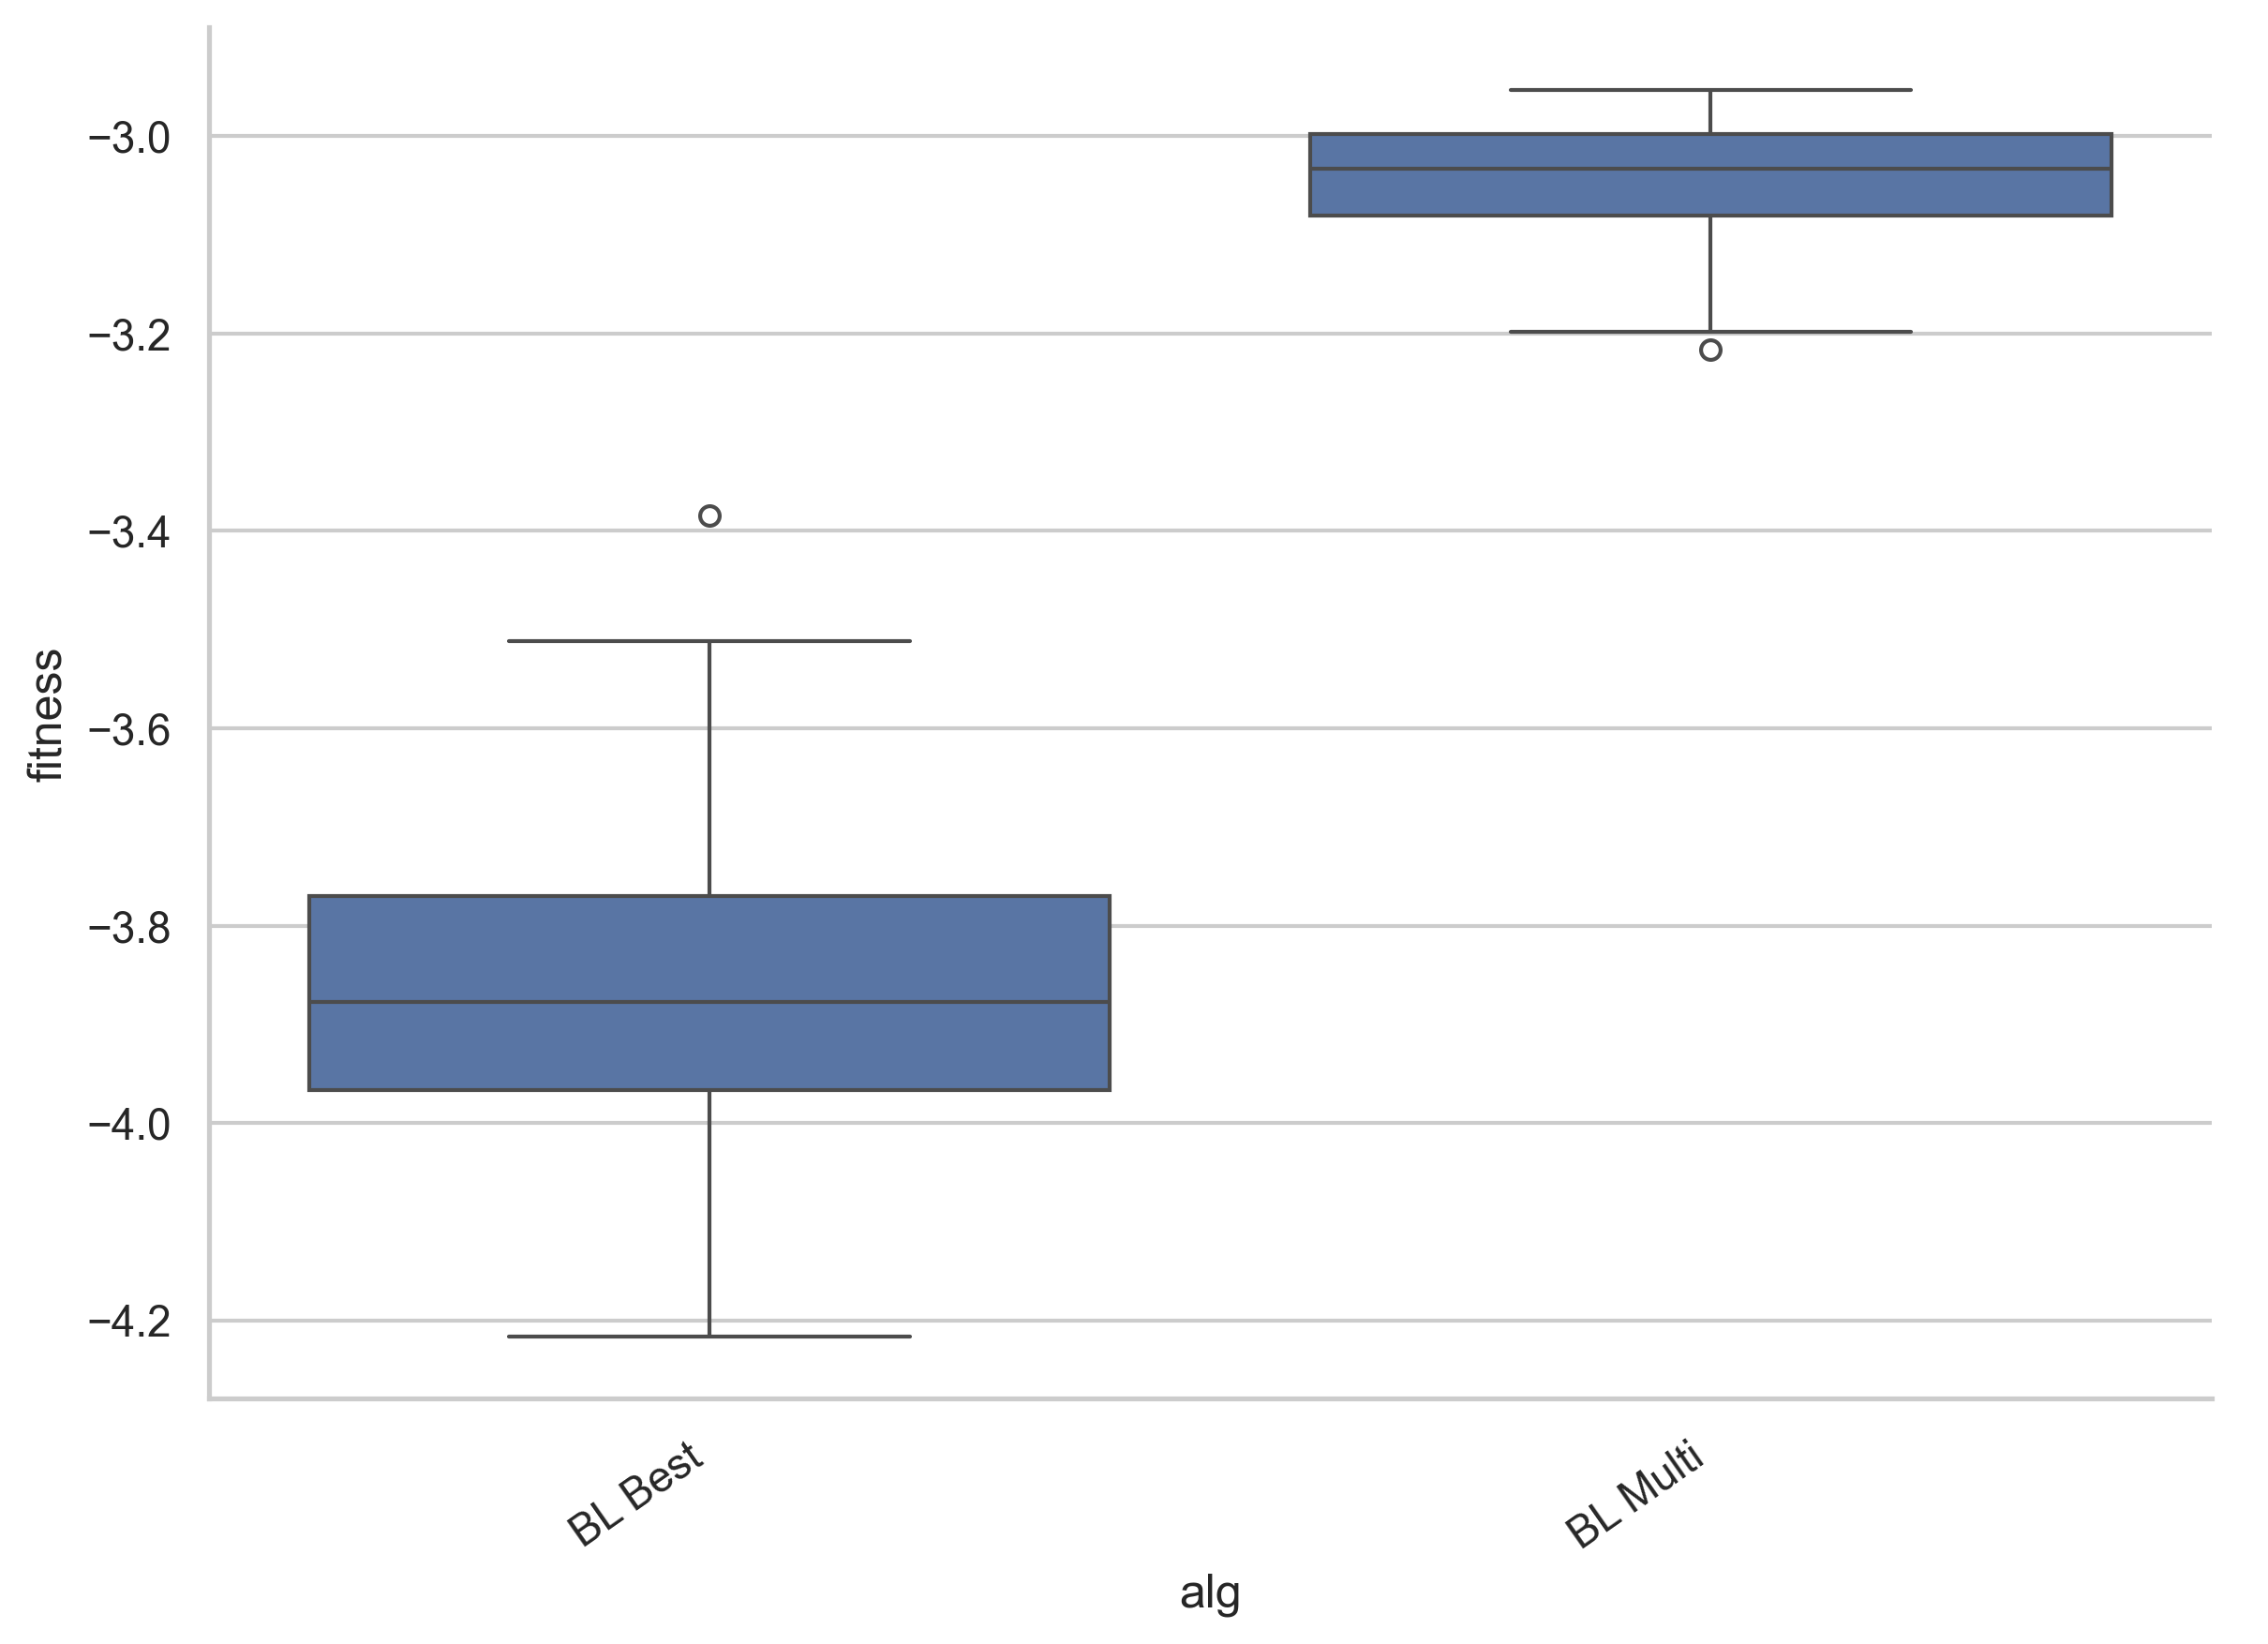
\includegraphics[width=0.85\textwidth]{figuras/S&P_100_RESULTS_pr1_extras.png}
    \caption{Boxplots de los extras de la Práctica 1 -- S\&P 100 (BL Best y BL Multi).}
    \label{fig:pr1-extras-sp100}
\end{figure}

\begin{figure}[H]
    \centering
    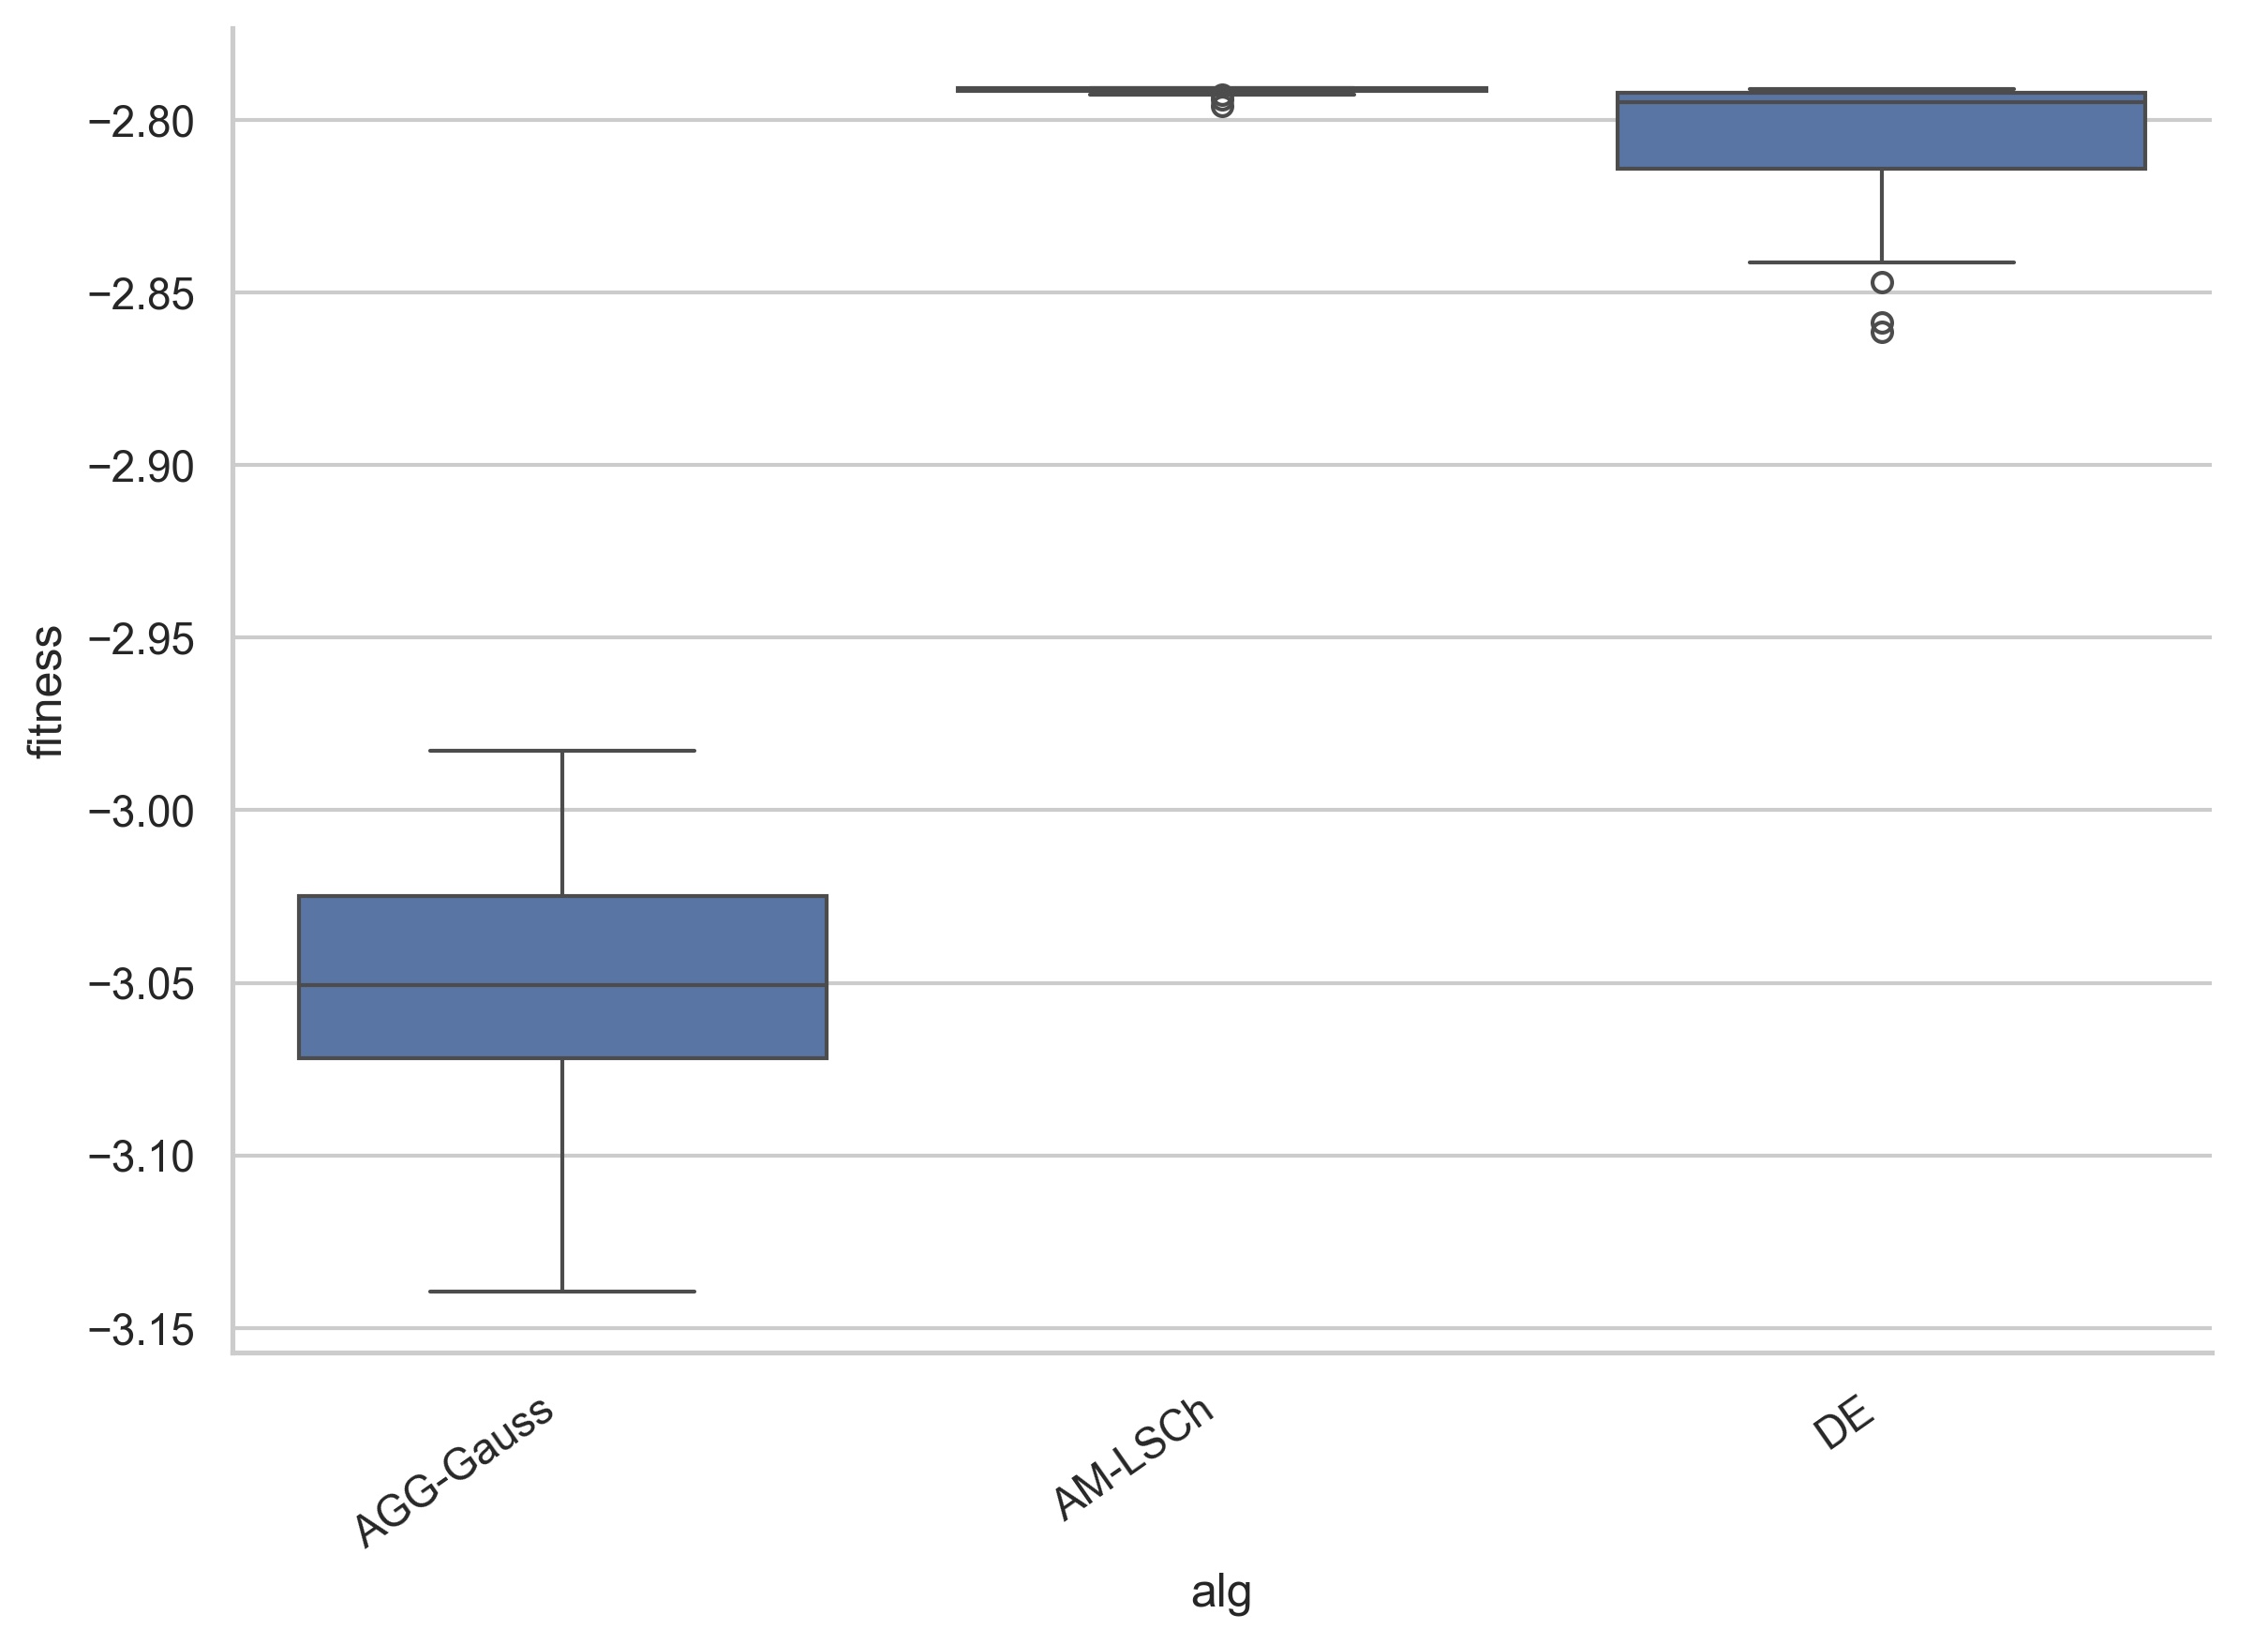
\includegraphics[width=0.85\textwidth]{figuras/S&P_100_RESULTS_pr2_extras.png}
    \caption{Boxplots de los extras de la Práctica 2 -- S\&P 100 (AGG-Gauss, AM-LSCh y DE).}
    \label{fig:pr2-extras-sp100}
\end{figure}

\begin{figure}[H]
    \centering
    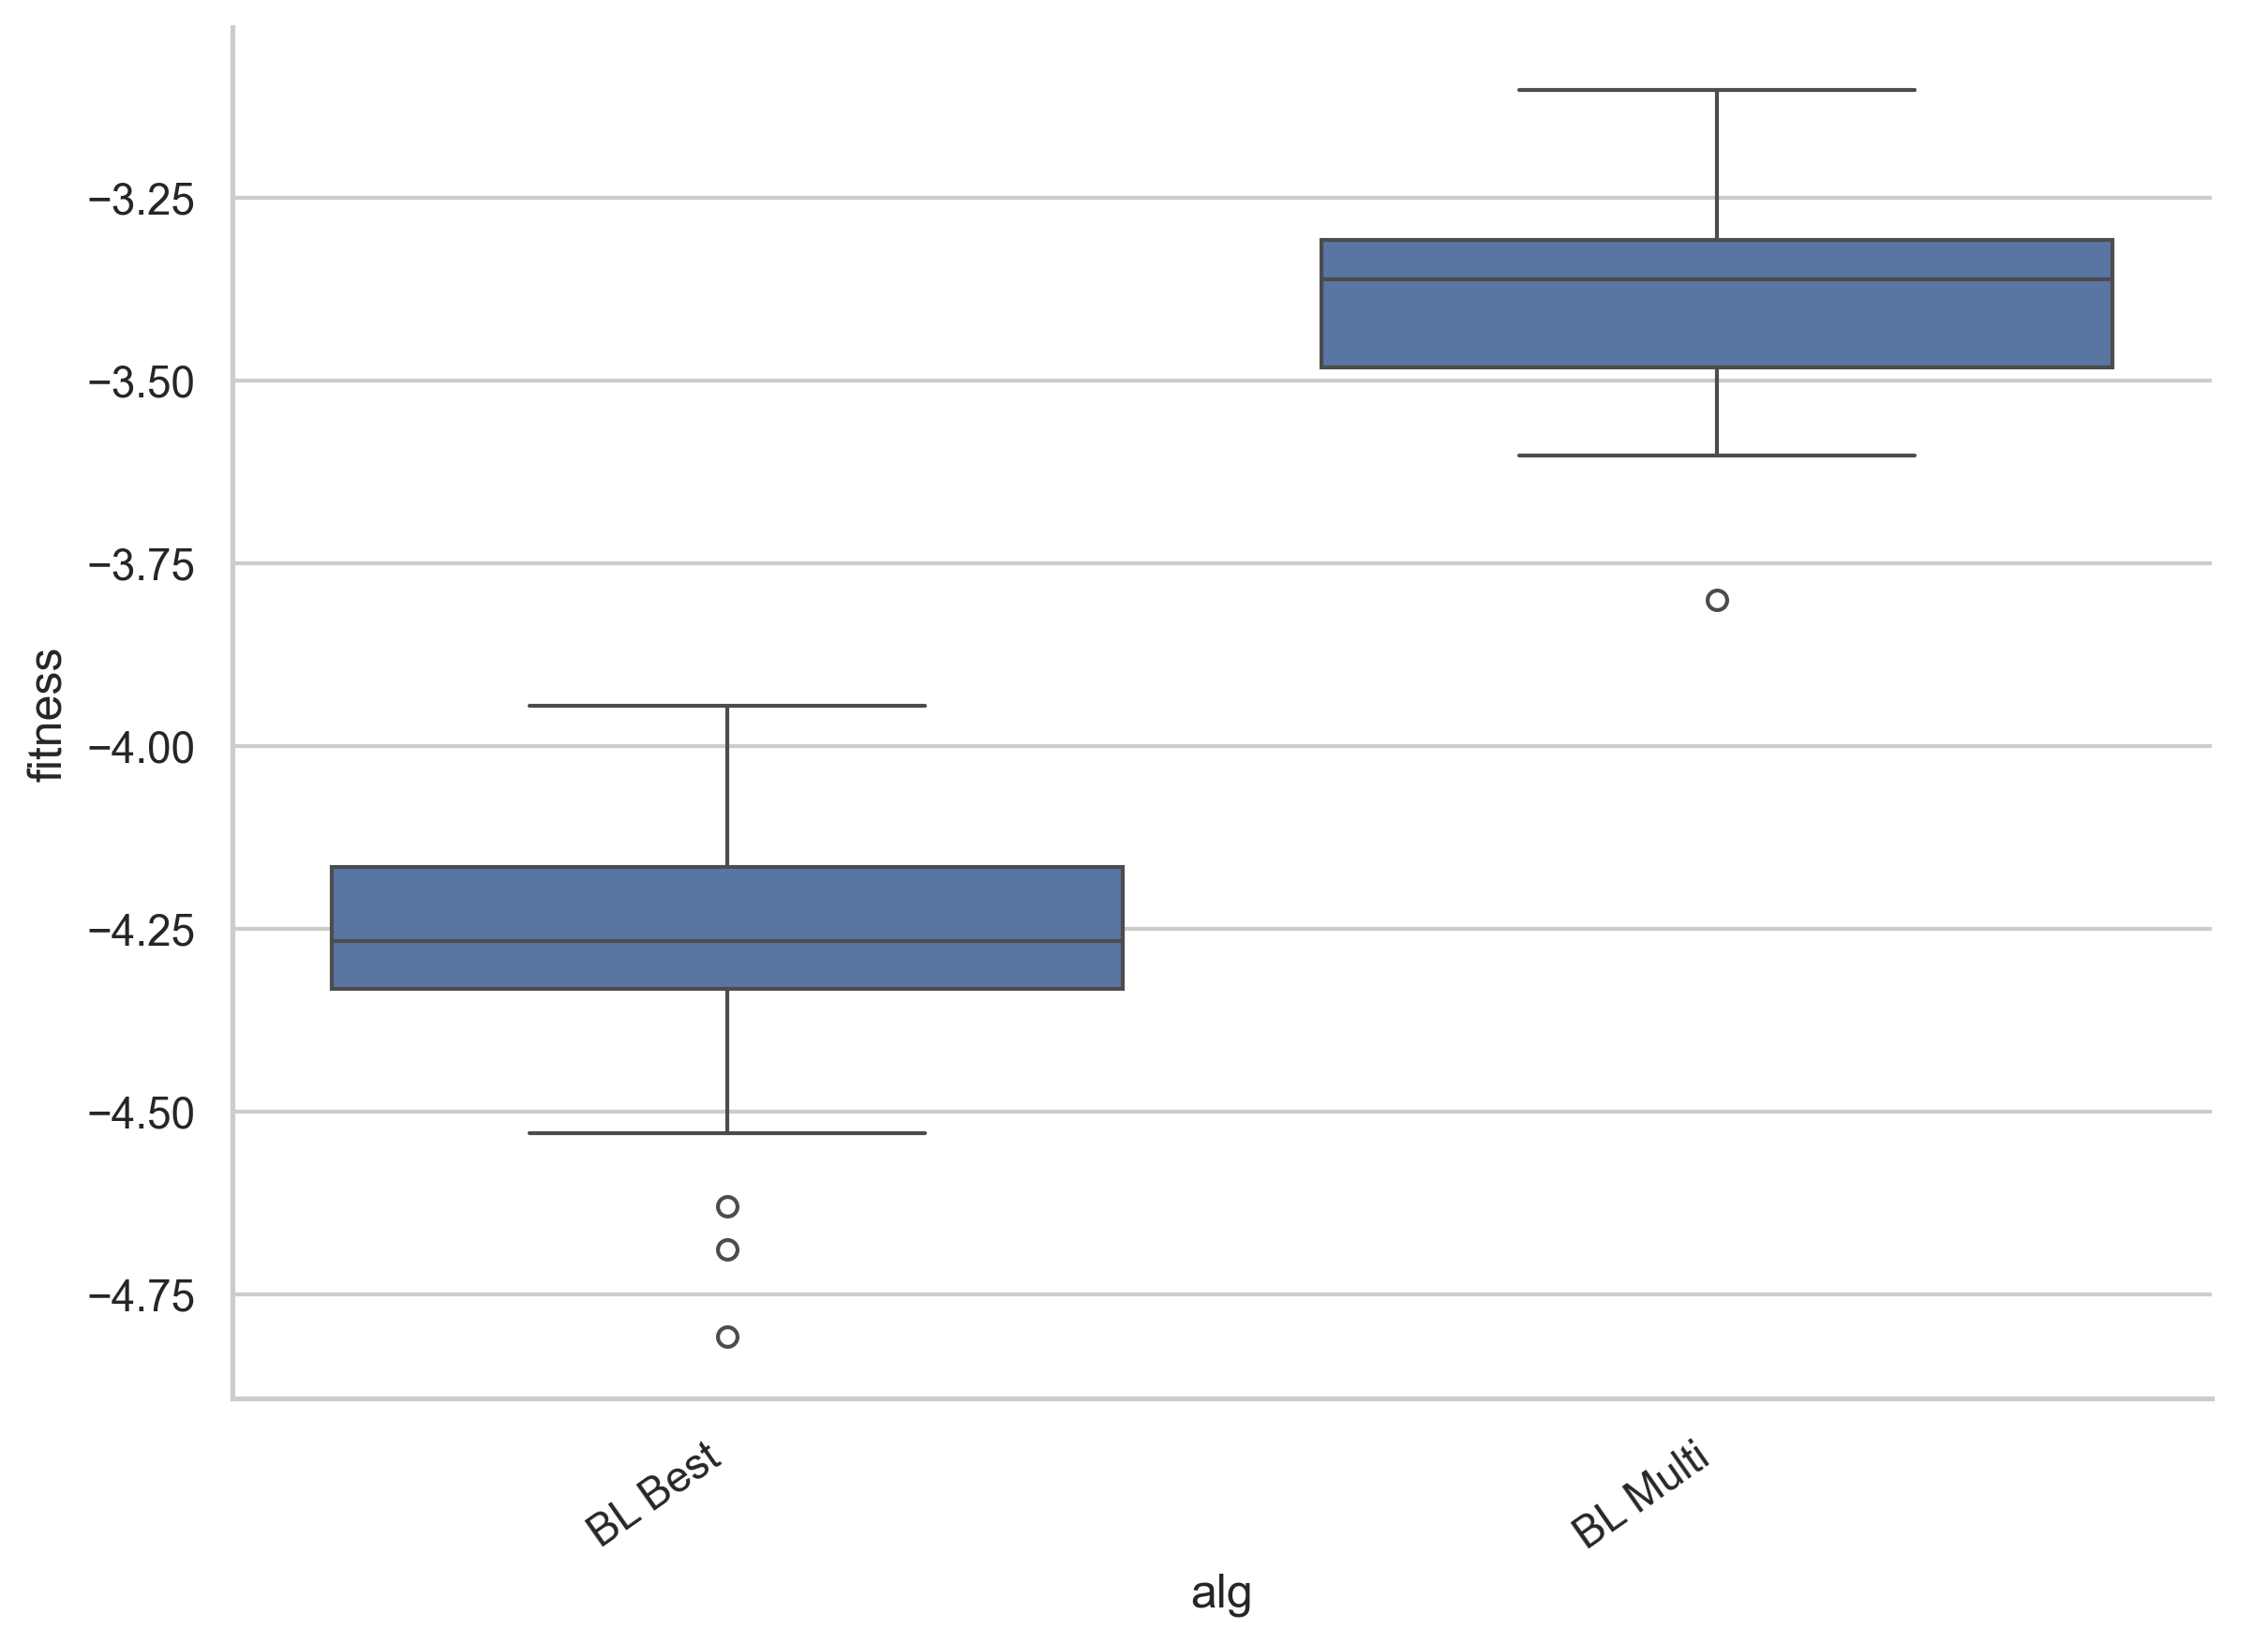
\includegraphics[width=0.85\textwidth]{figuras/S&P_500_RESULTS_pr1_extras.png}
    \caption{Boxplots de los extras de la Práctica 1 -- S\&P 500 (BL Best y BL Multi).}
    \label{fig:pr1-extras-sp500}
\end{figure}

\begin{figure}[H]
    \centering
    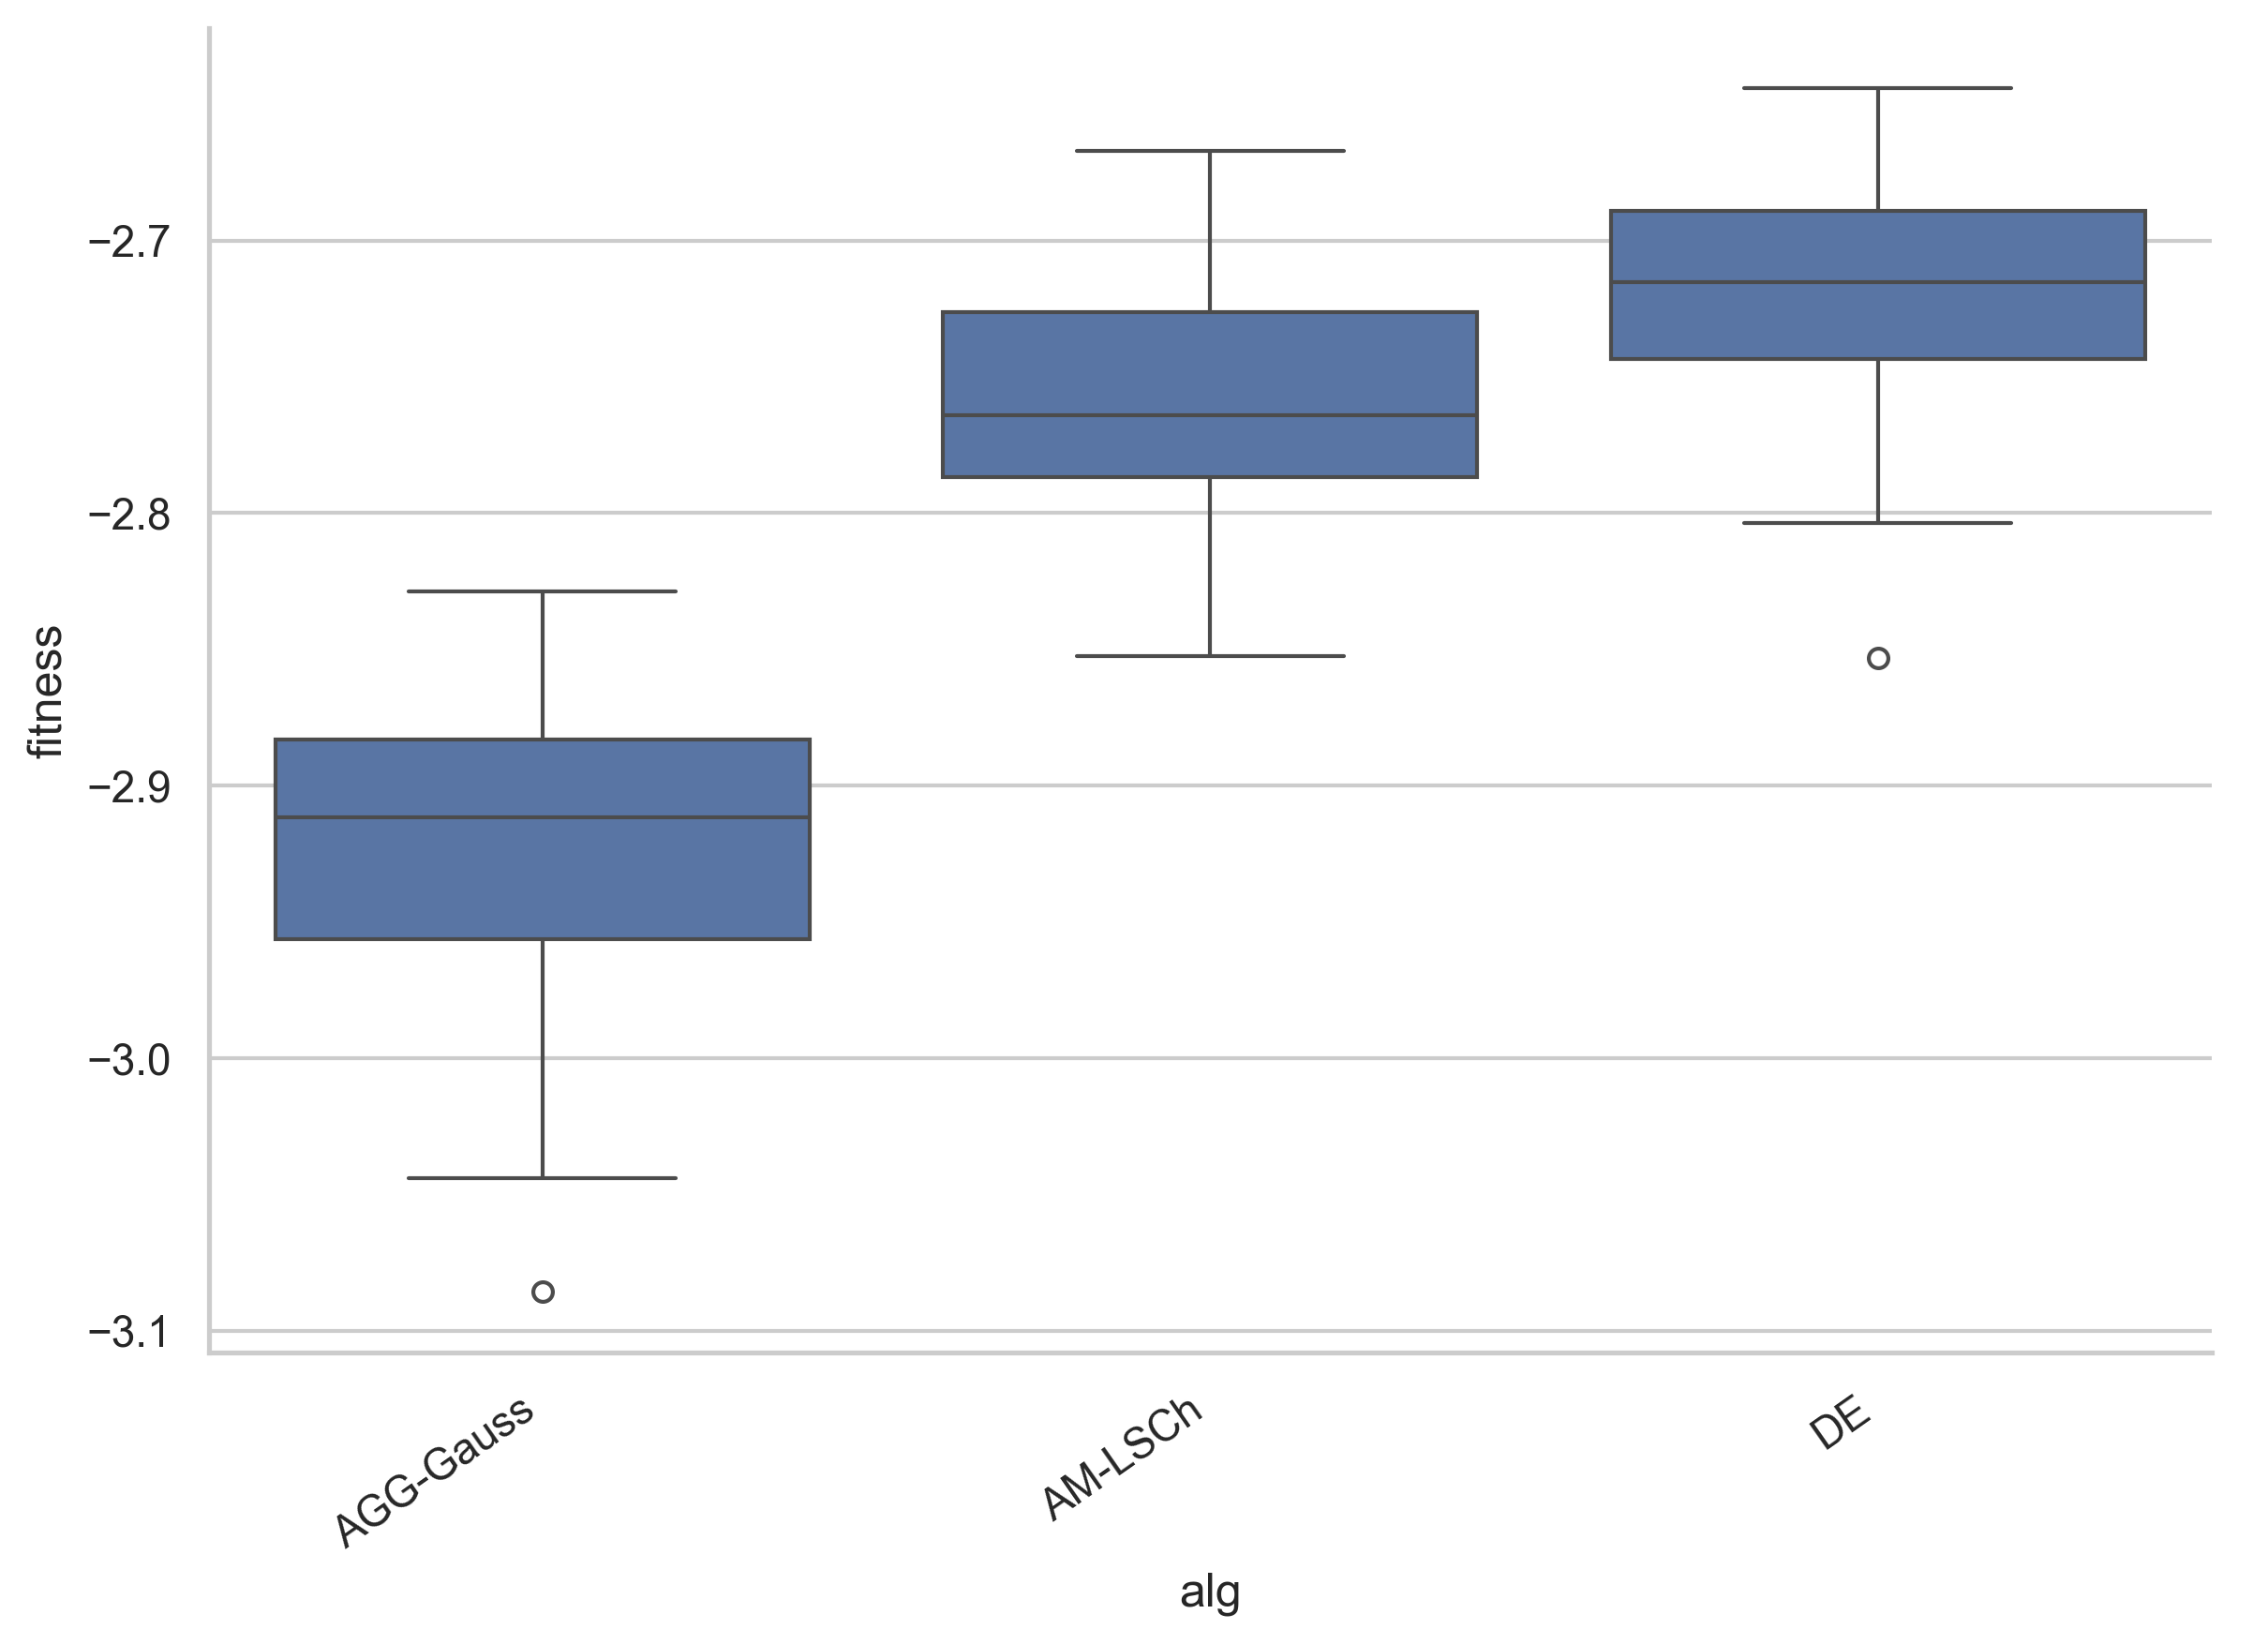
\includegraphics[width=0.85\textwidth]{figuras/S&P_500_RESULTS_pr2_extras.png}
    \caption{Boxplots de los extras de la Práctica 2 -- S\&P 500 (AGG-Gauss, AM-LSCh y DE).}
    \label{fig:pr2-extras-sp500}
\end{figure}

\subsection{Mutación Gaussiana en AGG}

\subsubsection{Pseudocódigo}

\begin{algorithm}[H]
\SetAlgoLined
\KwIn{Solución $S = (s_1, \dots, s_N)$, probabilidad de mutación por individuo $p_m$, desviación típica $\sigma$, límites $[lo, hi]$, tolerancia $\epsilon$}
\KwOut{Solución mutada y factible}

$S_{orig} \leftarrow S$\;
$p_{gen} \leftarrow \min\bigl(1,\; p_m / N\bigr)$\;
$mutado \leftarrow \textbf{false}$\;

\tcp{Fase 1: Perturbación gaussiana gen a gen}
\For{$i \leftarrow 1$ \KwTo $N$}{
    \If{$\text{rand}(0,1) \leq p_{gen}$}{
        \tcp{Ruido Box-Muller}
        $u_1 \leftarrow \text{rand}(10^{-12},\, 1)$\;
        $u_2 \leftarrow \text{rand}(0,\, 1)$\;
        $z \leftarrow \sqrt{-2\ln u_1}\,\cos(2\pi\, u_2)$\;
        $candidato \leftarrow s_i + z \cdot \sigma$\;
        \If{$candidato \in \{0\} \cup [lo,\, hi]$}{
            $s_i \leftarrow candidato$\;
            $mutado \leftarrow \textbf{true}$\;
        }
    }
}

\If{$\neg\, mutado$}{
    \Return $S$\;
}

\tcp{Fase 2: Reparación de la restricción $\sum s_i = 1$}
$\delta \leftarrow 1 - \sum_{i=1}^{N} s_i$\;

\If{$|\delta| \leq \epsilon$ \textbf{y} $S$ es válida}{
    \Return $S$\;
}

\tcp{Redistribuir $\delta$ en un gen aleatorio}
$indices \leftarrow$ permutación aleatoria de $\{1,\dots,N\}$\;
\For{$k \in indices$}{
    $valor\_anterior \leftarrow s_k$\;
    $candidato \leftarrow valor\_anterior + \delta$\;
    \If{$candidato \in \{0\} \cup [lo,\, hi]$}{
        $s_k \leftarrow candidato$\;
        \If{$S$ es válida}{
            \Return $S$\;
        }
        $s_k \leftarrow valor\_anterior$\;
    }
}

\tcp{Si no se pudo reparar, revertir}
\Return $S_{orig}$\;
\caption{Mutación Gaussiana}
\label{alg:gaussian-mutation}
\end{algorithm}

\subsubsection{Configuración experimental}

AGG-Gauss se construye sobre la estructura del AGG generacional obligatorio con \textbf{cruce aritmético}, sustituyendo únicamente el operador de mutación por transferencia por la perturbación gaussiana descrita. Los parámetros relevantes son:

\begin{itemize}[noitemsep]
    \item Desviación típica del ruido: $\sigma = 0{,}02$ (\texttt{GA\_GAUSSIAN\_SIGMA}).
    \item Probabilidad de mutación por individuo: $P_m = 0{,}1$ (heredada del AG base).
    \item Probabilidad por gen: $p_{gen} = \min\bigl(1,\; P_m / N\bigr)$, adaptativa al tamaño del mercado.
    \item Cruce, selección, elitismo y resto de parámetros: idénticos a AGG-Arit (véase Sección~\ref{sec:experimentos}).
\end{itemize}

\subsubsection{Análisis de AGG-Gauss}

La comparación más justa para evaluar el valor de la mutación gaussiana es frente a \textbf{AGG-Arit}, con el que comparte cruce y esquema generacional y solo difiere en el operador de mutación. Frente a este, AGG-Gauss obtiene una mejora consistente en todos los mercados: en torno al 3\,\% en el IBEX~35, cercana al 6\,\% en el S\&P~100 y de aproximadamente un 3\,\% en el S\&P~500. Esta ventaja se explica por la naturaleza de la perturbación: mientras la mutación por transferencia redistribuye una cantidad fija (15\,\%) de capital entre dos genes ---lo que genera saltos discretos y relativamente bruscos---, la mutación gaussiana aplica un ruido suave y continuo, permitiendo un refinamiento más granular del vector de pesos sin comprometer excesivamente la estructura de la solución.

Sin embargo, al comparar AGG-Gauss con \textbf{AGG-BLX}, la variante gaussiana queda ligeramente por debajo en los tres mercados: un 0,3\,\% en el IBEX~35, un 2\,\% en el S\&P~100 y cerca del 3\,\% en el S\&P~500. Esto pone de manifiesto que el beneficio de la perturbación gaussiana no logra compensar la ventaja estructural que confiere el cruce BLX-$\alpha$ sobre el cruce aritmético. El muestreo expandido de BLX genera una diversidad en la recombinación que resulta más decisiva para la calidad final que el tipo de mutación empleado, lo cual es coherente con la teoría: en los algoritmos genéticos la mutación cumple un papel secundario de mantenimiento de diversidad, mientras que el cruce es el operador principal de exploración.

Respecto a la \textbf{variabilidad}, los boxplots muestran que AGG-Gauss posee una dispersión intermedia. En el IBEX~35 su rango intercuartílico es más ancho que el de AGG-BLX pero más estrecho que el de AGG-Arit, sin presencia de outliers. En el S\&P~100 se observa un patrón similar, con una caja más contenida que la del cruce aritmético y sin valores atípicos. En el S\&P~500, AGG-Gauss amplía su dispersión y presenta un outlier inferior, indicando que en dimensiones altas la perturbación gaussiana puede conducir puntualmente a soluciones subóptimas cuando la reparación de factibilidad no consigue absorber el ruido acumulado en los $N=500$ genes.

En resumen, la mutación gaussiana constituye una mejora clara respecto a la mutación por transferencia sobre el mismo cruce aritmético, pero no resulta suficiente para superar el rendimiento del cruce BLX. La principal contribución de esta variante es demostrar que el operador de mutación sí influye en la calidad del AG, aunque su impacto es menor que el del operador de cruce.

\subsection{Algoritmo Memético Local Search Chains (AM-LSCh)}

\subsubsection{Pseudocódigo}

\newpage
\scalebox{0.84}{\begin{minipage}{1.19\textwidth}
\begin{algorithm}[H]
\SetAlgoLined
\KwIn{Problema $P$, presupuesto $maxEvals$, población $|Pop|$, $P_c$, $P_m$, periodo BL $T$, ratio $r$, intensidad $I_{str}$}
\KwOut{Mejor solución encontrada}

$evals \leftarrow 0$, $gen \leftarrow 0$\;
$Pop \leftarrow$ inicializar población de $|Pop|$ individuos (evaluar, actualizar $evals$)\;
$Estado[i] \leftarrow \emptyset \;\forall i$\;
\tcp{Estado BL vacío por individuo}
$mejor \leftarrow$ mejor individuo de $Pop$\;

\While{$evals + |Pop| \leq maxEvals$}{

    \tcp{Selección: torneo de tamaño 3}
    \For{$i \leftarrow 1$ \KwTo $|Pop|$}{
        $idx\_padre[i] \leftarrow$ Torneo$_3$($Pop$)\;
        $Padres[i] \leftarrow Pop[idx\_padre[i]]$\;
    }

    \tcp{Cruce: número esperado de parejas cruzadas}
    $n_{cruces} \leftarrow \lfloor P_c \cdot |Pop|/2 \rfloor$\;
    \For{$p \leftarrow 1$ \KwTo $|Pop|/2$}{
        $i \leftarrow 2p-1$, $j \leftarrow 2p$\;
        \eIf{$p \leq n_{cruces}$}{
            $(Hijos[i],\, Hijos[j]) \leftarrow$ Cruce($Padres[i]$, $Padres[j]$)\;
            Resetear $Estado\_hijo[i]$ y $Estado\_hijo[j]$\;
        }{
            $Hijos[i] \leftarrow Padres[i]$, $Hijos[j] \leftarrow Padres[j]$\;
            $Estado\_hijo[i] \leftarrow Estado[idx\_padre[i]]$\;\tcp*{Hereda cadena}
            $Estado\_hijo[j] \leftarrow Estado[idx\_padre[j]]$\;
        }
    }

    \tcp{Mutación: número esperado de individuos mutados}
    $n_{mut} \leftarrow \lfloor P_m \cdot |Pop| \rfloor$\;
    Seleccionar $n_{mut}$ índices aleatorios sin repetición\;
    \For{cada índice $k$ seleccionado}{
        Mutar $Hijos[k]$ por transferencia\;
        Resetear $Estado\_hijo[k]$\;
    }

    Evaluar todos los hijos (actualizar $evals$)\;
    $mejor\_prev \leftarrow$ mejor de $Pop$ antes del reemplazo\;
    $Pop \leftarrow Hijos$, $Estado \leftarrow Estado\_hijo$\;
    $gen \leftarrow gen + 1$\;

    \tcp{BL encadenada: solo al mejor, cada $T$ generaciones}
    \If{$T > 0$ \textbf{y} $gen \bmod T = 0$}{
        $idx \leftarrow$ índice del mejor de $Pop$\;
        $budget \leftarrow \min(I_{str},\; maxEvals - evals)$\;
        \If{$budget > 0$}{
            $usadas \leftarrow$ BL-Encadenada($P$, $Pop[idx]$, $r$, $budget$, $Estado[idx]$)\;
            $evals \leftarrow evals + usadas$\;
        }
    }

    \tcp{Elitismo: preservar mejor de generación anterior}
    \If{$f(mejor\_prev) > f($mejor de $Pop)$}{
        Reemplazar peor de $Pop$ por $mejor\_prev$ (y su estado)\;
    }

    Actualizar $mejor$ global si $Pop$ contiene uno superior\;
}
\Return $mejor$\;
\caption{AM-LSCh: Memético con Cadenas de Búsqueda Local}
\label{alg:am-lsch}
\end{algorithm}
\end{minipage}}

\vspace{0.5em}

\begin{algorithm}[H]
\SetAlgoLined
\KwIn{Problema $P$, solución $S$, fitness $f$, ratio $r$, presupuesto $budget$, estado $\mathcal{E}$ ($c$, $V$, $d$)}
\KwOut{Evaluaciones consumidas; $S$ y $f$ actualizados \textit{in-place}}

\tcp{Inicialización lazy del estado}
\If{$d \neq |S|$ \textbf{o} $V = \emptyset$}{
    $V \leftarrow$ todos los pares $(i,j)$ con $i \neq j$, barajados aleatoriamente\;
    $c \leftarrow 0$, $d \leftarrow |S|$\;
}

$evals \leftarrow 0$, $sin\_mejora \leftarrow 0$\;

\While{$evals < budget$ \textbf{y} $sin\_mejora < |V|$}{
    $(i, j) \leftarrow V[c]$\;
    $c \leftarrow (c + 1) \bmod |V|$\;
    $sin\_mejora \leftarrow sin\_mejora + 1$\;

    \If{$s_i = 0$}{\textbf{continuar}\;}

    $transfer \leftarrow s_i \cdot r$\;
    $s'_i \leftarrow s_i - transfer$, $s'_j \leftarrow s_j + transfer$\;

    \If{$s'_i \notin \{0\} \cup [lo,\, hi]$ \textbf{o} $s'_j \notin \{0\} \cup [lo,\, hi]$}{
        \textbf{continuar}\;
    }

    $S' \leftarrow S$ con $s'_i$ y $s'_j$\;
    $f' \leftarrow fitness(S')$, $evals \leftarrow evals + 1$\;

    \If{$f' > f$}{
        $S \leftarrow S'$, $f \leftarrow f'$\;
        $sin\_mejora \leftarrow 0$\tcp*{Primer mejora: resetear contador}
    }
}
\Return $evals$\;
\caption{BL-Soft-Encadenada (con estado persistente)}
\label{alg:soft-ls-chain}
\end{algorithm}

\subsubsection{Configuración experimental}

AM-LSCh hereda la base generacional del AGG con el \textbf{mejor cruce} seleccionado automáticamente (BLX-$\alpha$ en todos los mercados). Los parámetros específicos de la cadena de búsqueda local son:

\begin{itemize}[noitemsep]
    \item Intensidad por invocación: $I_{str} = 500$ evaluaciones (\texttt{AM\_LSCH\_I\_STR}).
    \item Frecuencia: cada $T = 10$ generaciones (\texttt{AM\_LS\_PERIOD}).
    \item Ratio de transferencia de la BL: $r = 0{,}15$ (\texttt{AM\_LS\_RATIO}).
    \item Aplicación: exclusivamente al \textbf{mejor individuo} de la población.
    \item Resto de parámetros ($|Pop|=100$, $P_c=0{,}8$, $P_m=0{,}1$, $\alpha=0{,}3$): heredados del AGG base.
\end{itemize}

La diferencia clave frente a los meméticos obligatorios es doble: (1) la BL se aplica solo al élite, no a un subconjunto de la población; y (2) el estado de exploración del vecindario \textbf{persiste entre generaciones}, lo que evita revisitar movimientos ya descartados.

\subsubsection{Análisis de AM-LSCh}

La comparación natural de AM-LSCh es frente a \textbf{AM-Best} y \textbf{AM-Rand}, que son las variantes obligatorias con mejor rendimiento. En el IBEX~35, las tres variantes alcanzan medias prácticamente idénticas, lo que indica que en mercados pequeños ($N=35$) la intensificación adicional del encadenamiento no aporta una ventaja significativa: el espacio de búsqueda es lo suficientemente reducido para que la BL estándar ya converja con eficacia. En el S\&P~100, AM-LSCh mejora ligeramente a AM-Best (en torno al 1\,\%) y a AM-Rand (cerca del 1{,}1\,\%), una ganancia modesta pero consistente que se explica por la eficiencia del cursor persistente, que aprovecha mejor el presupuesto de $I_{str}=500$ evaluaciones al no repetir zonas ya exploradas del vecindario.

En el S\&P~500, sin embargo, AM-LSCh queda aproximadamente un 1\,\% por detrás de AM-Rand y AM-Best. Este resultado, aparentemente contradictorio, tiene una explicación estructural: con $N=500$ genes, el vecindario completo contiene $500 \times 499 = 249\,500$ movimientos posibles. Un presupuesto fijo de 500 evaluaciones por invocación explora apenas el 0{,}2\,\% de ese vecindario, lo que reduce drásticamente la probabilidad de encontrar movimientos de mejora dentro de una sola cadena. En contraste, AM-Rand y AM-Best aplican la BL a varios individuos con vecindarios independientes, lo que genera una exploración efectiva más diversa.

Frente a \textbf{AM-All}, AM-LSCh es claramente superior en todos los mercados: un 2\,\% en el IBEX~35, un 10\,\% en el S\&P~100 y cerca del 14\,\% en el S\&P~500. Esto confirma que la aplicación exhaustiva de BL a toda la población (AM-All) constituye un desperdicio de evaluaciones que degrada el rendimiento global, mientras que la focalización en el élite ---ya sea con cadenas o con las variantes Rand/Best--- es una estrategia mucho más rentable.

Respecto a la \textbf{variabilidad}, AM-LSCh destaca por una desviación estándar extraordinariamente baja, lo que provoca que los boxplots colapsen a una línea horizontal en los tres mercados. En el IBEX~35, la caja se reduce a un trazo con un único outlier justo en la línea, fruto de una ejecución que convergió a un valor marginalmente distinto. En el S\&P~100, el patrón es análogo pero con varios outliers sobre la misma línea, evidenciando que unas pocas ejecuciones difirieron mínimamente del valor dominante. En el S\&P~500, en cambio, no se observa ningún outlier: la dispersión general es algo mayor (la caja deja de ser un trazo puro), pero todas las ejecuciones se mantienen dentro del rango intercuartílico sin desviaciones anómalas.

\subsection{Evolución Diferencial (DE)}

\subsubsection{Pseudocódigo}

\begin{algorithm}[H]
\SetAlgoLined
\KwIn{Problema $P$, presupuesto $maxEvals$, población $|Pop|$, factor de mutación $F$, tasa de cruce $CR$}
\KwOut{Mejor solución encontrada}

\tcp{Ajuste dinámico del tamaño de población}
$|Pop| \leftarrow \max\bigl(20,\; \min(|Pop|,\; \max(20,\; \lfloor maxEvals/4 \rfloor))\bigr)$\;

$evals \leftarrow 0$\;
$Pop \leftarrow$ inicializar $|Pop|$ individuos aleatorios (evaluar, actualizar $evals$)\;
$mejor \leftarrow$ mejor individuo de $Pop$\;

\While{$evals < maxEvals$}{
    \For{$i \leftarrow 1$ \KwTo $|Pop|$}{
        \If{$evals \geq maxEvals$}{\textbf{salir}\;}

        \tcp{Mutación diferencial: DE/rand/1}
        Seleccionar $r_0, r_1, r_2$ distintos entre sí y distintos de $i$\;
        \For{$d \leftarrow 1$ \KwTo $N$}{
            $donor_d \leftarrow x_{r_0,d} + F \cdot (x_{r_1,d} - x_{r_2,d})$\;
        }

        \tcp{Cruce binomial}
        $trial \leftarrow x_i$\;
        $j_{rand} \leftarrow$ índice aleatorio en $\{1,\dots,N\}$\;
        \For{$d \leftarrow 1$ \KwTo $N$}{
            \If{$\text{rand}(0,1) \leq CR$ \textbf{o} $d = j_{rand}$}{
                $trial_d \leftarrow donor_d$\;
            }
        }

        Reparar $trial$ (forzar factibilidad)\;
        $f_{trial} \leftarrow fitness(trial)$, $evals \leftarrow evals + 1$\;

        \tcp{Selección determinista}
        \If{$f_{trial} > f_i$}{
            $x_i \leftarrow trial$, $f_i \leftarrow f_{trial}$\;
            \If{$f_{trial} > f(mejor)$}{
                $mejor \leftarrow x_i$\;
            }
        }
    }
}
\Return $mejor$\;
\caption{Evolución Diferencial (DE/rand/1/bin)}
\label{alg:de}
\end{algorithm}

\subsubsection{Configuración experimental}

La implementación sigue el esquema clásico \textbf{DE/rand/1/bin}: mutación diferencial con un vector base aleatorio y un par de diferencia, seguida de cruce binomial y selección determinista. Los parámetros son:

\begin{itemize}[noitemsep]
    \item Factor de escala: $F = 0{,}5$ (\texttt{DE\_F}).
    \item Tasa de cruce binomial: $CR = 0{,}9$ (\texttt{DE\_CR}).
    \item Tamaño de población: $|Pop| = 100$ (\texttt{DE\_POP\_SIZE}), con ajuste dinámico que garantiza un mínimo de 20 individuos y al menos 4 generaciones completas.
    \item Reparación de factibilidad: se aplica únicamente al vector \textit{trial} tras el cruce, no al vector \textit{donor}, para preservar la geometría del paso diferencial.
\end{itemize}

Un aspecto notable de la implementación es que el vector \textit{donor} no se repara antes del cruce. Esto es deliberado: la diferencia $(x_{r_1} - x_{r_2})$ actúa como un vector de dirección puro, y recortarla prematuramente alteraría la dinámica adaptativa de DE, en la que el tamaño de paso se autorregula según la dispersión de la población.

\subsubsection{Análisis de DE}

DE obtiene resultados competitivos frente a los mejores algoritmos obligatorios. En el IBEX~35, su fitness medio es prácticamente idéntico al de AM-Best y AM-Rand, lo que confirma que en mercados pequeños ($N=35$) la mayoría de los algoritmos poblacionales convergen al mismo óptimo. En el S\&P~100, DE mejora a AGG-BLX en torno al 3\,\% y se sitúa a menos del 0{,}5\,\% de AM-Best, un resultado notable considerando que DE no incorpora ninguna fase de búsqueda local explícita.

El resultado más destacado se produce en el \textbf{S\&P~500}, donde DE alcanza el mejor fitness medio de todos los algoritmos evaluados, superando a AM-Rand en aproximadamente un 0{,}6\,\% y a AGG-BLX en un 3\,\%. Esta ventaja se explica por la naturaleza del operador de mutación diferencial: el paso $F \cdot (x_{r_1} - x_{r_2})$ es inherentemente adaptativo al espacio de búsqueda, ya que su magnitud escala con la diversidad de la población. En dimensiones altas ($N=500$), esta propiedad resulta especialmente valiosa porque permite explorar direcciones geométricamente relevantes sin necesidad de un vecindario explícito de $N \times (N-1)$ movimientos como en la búsqueda local.

Frente a \textbf{AGG-Gauss}, DE es consistentemente superior: un 2\,\% en el IBEX~35, un 5\,\% en el S\&P~100 y un 6\,\% en el S\&P~500. Ambos operadores trabajan con perturbaciones continuas, pero la mutación diferencial tiene la ventaja de ser \textit{informada} por la estructura de la población (usa diferencias reales entre individuos), mientras que la gaussiana aplica ruido ciego independiente de la distribución actual.

Respecto a la \textbf{variabilidad}, DE muestra una desviación estándar baja en el IBEX~35 y el S\&P~100, comparable a la de los algoritmos meméticos. En el S\&P~500 su dispersión es moderada, similar a la de AM-LSCh. En cuanto a los boxplots, no se aprecia ningún outlier en el IBEX~35, el S\&P~100 muestra alguno sobre una caja compacta y el S\&P~500 presenta un boxplot limpio sin valores atípicos.

\subsection{Comparación global de los extras}

Los cinco algoritmos extras comparten el mismo presupuesto de 10\,000 evaluaciones y las mismas instancias, por lo que su comparación directa es metodológicamente legítima a pesar de pertenecer a paradigmas distintos. El ranking general de fitness medio, de mejor a peor, es:

\begin{enumerate}[noitemsep]
    \item \textbf{DE} y \textbf{AM-LSCh}: ocupan las dos primeras posiciones de forma alternante. DE domina en el S\&P~500, AM-LSCh en el S\&P~100, y ambos empatan virtualmente en el IBEX~35.
    \item \textbf{AGG-Gauss}: tercera posición, mejorando al cruce aritmético estándar pero sin alcanzar a los dos anteriores.
    \item \textbf{BL Multi}: cuarta posición, con un rendimiento razonable en el IBEX~35 pero que se degrada notablemente al crecer la dimensión.
    \item \textbf{BL Best}: última posición en todos los mercados, con diferencias de más del 30\,\% en el S\&P~500 respecto a DE.
\end{enumerate}

Respecto a las \textbf{búsquedas locales de la Práctica~1} (BL Best y BL Multi), su inclusión como extras tiene un propósito comparativo: evidenciar la brecha entre métodos de trayectoria simple y métodos poblacionales bajo el mismo presupuesto. BL Best, al partir de un único punto y explorar un vecindario de primer mejora, carece de diversificación y queda atrapada en óptimos locales prematuros, especialmente en dimensiones altas. BL Multi mitiga parcialmente este problema mediante reinicios aleatorios, pero la calidad de cada reinicio depende del azar de la inicialización y no hay comunicación entre las distintas trayectorias. En contraste, los tres extras de la Práctica~2 mantienen una población que intercambia información geométrica (vía cruce, mutación diferencial o búsqueda local encadenada), lo que les confiere una exploración estructuralmente más eficiente.

En definitiva, la comparación confirma que los enfoques poblacionales ---y en particular DE y AM-LSCh--- aprovechan mejor el presupuesto de evaluaciones que las búsquedas locales aisladas, y que la ventaja se amplifica a medida que crece la dimensionalidad del problema.

\subsection{Anotaciones sobre la Parametrización}

En las implementaciones que hemos discutido (como el Algoritmo Memético, la Búsqueda Local y el modelo AM-LSCh), varios de los parámetros y variables se eligieron siguiendo recomendaciones directas de la literatura científica y estudios empíricos. Estos son los principales y sus respectivos estudios:

\begin{enumerate}
    \item \textbf{La intensidad fija $I_{str} = 500$ en AM-LSCh:}
    En el modelo de Cadenas de Búsqueda Local (AM-LSCh), la intensidad de la búsqueda o \textit{LS intensity stretch} ($I_{str}$) se fija en 500 evaluaciones por eslabón. Esta decisión proviene del artículo original \textit{``Memetic Algorithms for Continuous Optimization Based on Local Search Chains''}, publicado por D. Molina, M. Lozano, C. García-Martínez y F. Herrera en la revista \textit{Evolutionary Computation} en 2010. En sus análisis experimentales sobre múltiples dimensiones, los autores demostraron concluyentemente que \textbf{``$I_{str} = 500$ es la mejor elección''} (\textit{is the best choice}) para maximizar el rendimiento del algoritmo.

    \item \textbf{El parámetro de cruce $\alpha = 0{,}5$ en BLX-$\alpha$:}
    El cruce BLX-$\alpha$ define un intervalo de exploración matemática basado en la distancia entre los genes de los padres. La teoría de la computación evolutiva subraya que \textbf{los autores originales de este operador reportaron los mejores resultados utilizando $\alpha = 0{,}5$}. Con este valor exacto, es estadísticamente igual de probable que el valor del hijo caiga dentro del rango cerrado de los padres como que caiga fuera, equilibrando perfectamente la exploración y la explotación. De hecho, el estudio de Molina et al. (2010) mencionado anteriormente también aplica el cruce BLX-$\alpha$ usando $\alpha = 0{,}5$ en su configuración estándar para el AM-LSCh, aunque en el guion básico de prácticas de Algoritmos Genéticos se recomendó probar con $\alpha = 0{,}3$.

    \item \textbf{El tamaño de transferencia en la Búsqueda Local (\texttt{ratio} = 0{,}4):}
    Para el problema de inversión del Portfolio, la metaheurística genera vecinos quitando un porcentaje a una empresa para dárselo a otra. El guion de la práctica establece explícitamente el uso de un \textbf{\texttt{ratio} = 0{,}4 (transferencia del 40\,\%)} porque, según el texto, \textbf{``es el valor más recomendado en la literatura''} para este tipo específico de exploración de entornos. \textit{(Cabe destacar que luego, en el Algoritmo Memético, bajamos este valor a 0{,}15 para lograr una ``Búsqueda Local Suave'' que fuera menos disruptiva con el genotipo).}

    \item \textbf{Probabilidad de selección para la Búsqueda Local ($P_{LS} = 0{,}1$ / 10\,\%):}
    En las variantes AM-Rand y AM-Best, aplicamos la Búsqueda Local únicamente al 10\,\% de la población cada 10 generaciones. La justificación teórica detrás de limitar esta variable al 10\,\% radica en las heurísticas de diseño para Algoritmos Meméticos: aplicar optimizadores locales sobre \textbf{un subconjunto muy acotado ayuda a no desbalancear severamente el equilibrio entre la exploración (búsqueda global) y la explotación (precisión local)}. Un porcentaje mayor destruiría la diversidad genética prematuramente.
\end{enumerate}
